
% TODO: somewhere in this chapter, I should do the parachute illustration with
% the gravitational force and the cross-wind force and the momentum from the
% airplane force. But where?

\chapter{Vectors}

\index{vector}
As I stated on p.~\pageref{mathematicalObject}, every ``algebra'' is comprised
of a set of mathematical objects which you can combine with various operations.
In linear algebra, those building blocks are \textbf{vector}s and
\textbf{matrices} (singular: matrix). Buried within them are many mysteries.
We'll cover them in considerable detail in this chapter and the next.

\section{Vector vs.~scalar quantities}

\index{scalar}
\index{scale of measure}

The first thing we should do is perhaps distinguish between a vector quantity
and a \textbf{scalar quantity}, which probably had the spotlight in most of
your previous math classes. A scalar value is simply a \textit{single} number,
like 5, or -3.2, or $\pi$, or even $9 + 2i$ if you're into imaginary numbers.
The word \textit{scalar} is related to the word \textit{scale}, as in a ``scale
of measure.'' Think of stepping on a scale to weigh yourself in the morning:
your scale gives you back a single number (which you may or may not like; I
won't judge).

\index{one-dimensional quantity}
\index{dimension}

We'll call scalars \textbf{one-dimensional} values. That might seem odd, since
we haven't really talked about ``dimensions,'' yet. But think of the plain-old
\textbf{number line} you learned about back in elementary school. Zero's drawn
in the middle, positive numbers to the right and negative numbers to the left,
and the whole thing extends infinitely in just one direction\footnote{It might
seem like ``two directions,'' since the number line goes both to the left and
to the right. But since \index{left-ness} \index{right-ness} left-ness is the
exact opposite of right-ness, these are considered ``the same direction''; it's
just a matter of how far you go back or forth you go along that one straight
path.}.

% TODO: draw number line

\index{tuna fish}
\index{stock price}

Examples are so ubiquitous they're hardly worth mentioning. A person's weight
in the morning is a scalar. A company's stock price on a given day is a scalar.
So is the net \textit{movement} (up or down) of a stock's price from one day to
the next. So is a respondent's answer to the survey question ``on a 1-to-10
scale, how much do you enjoy tuna fish?'' You can think of countless others.

We of course often use variables to represent scalar quantities, and in this
book we'll put a variable in italics (like ``\textit{x}'' or
``\textit{price}'') to signify that its underlying value is a scalar quantity.

\subsection{A vector: a multi-dimensional quantity}
\index{vector}

Now a vector quantity is kind of the same thing, except that it represents
\textit{more than one} value. Suppose we wanted to represent not just a stock's
price on a given day, but an entire year's worth of prices on consecutive days.
Then, we would need a vector quantity. Instead of a survey respondent's answer
to just one question, we might want to store her entire set of answers to all
twenty questions on the survey. Instead of tracking just my weight, I might
want to record my weight, height, BMI (body-mass index), and pulse, all at a
given moment.

\index{losing information}
\index{information loss}

Vectors are \textbf{multi-dimensional} quantities. And they can't be
represented on a number line. Let's say my weight is 210 lbs.~and my height is
6'2", or 74 inches. (This is not theoretical.) I could of course draw a number
line and put a dot at 74 and another dot at 210, but this wouldn't fully
represent the fact that my weight was 210 and my height was 74. For one thing,
the numbers are on completely different scales. (There's that word ``scale''
again.) For another, it's not clear which is which -- is the right-most point
supposed to be my height, or my weight? Trying to squeeze a two-dimensional
quantity into a one-dimensional number line would \textbf{lose information.}
We need a representation scheme that can accommodate the complexity of our
quantity.

\index{Cartesian plane}
\index{coordinate plane}

For a two-dimensional quantity like weight-and-height, the obvious choice is
the two-dimensional Cartesian plane. I've drawn the vector with my height and
weight on the left side of Figure~\ref{fig:vector}. You'll see that there's an
\textit{arrow} from the origin to the point (210,74), rather than just a
circular dot at that point, as you might have expected. This is because
sometimes, it turns out, we want to treat a vector as ``a net movement in a
particular direction for a particular distance.''


\begin{figure}[ht]
\centering
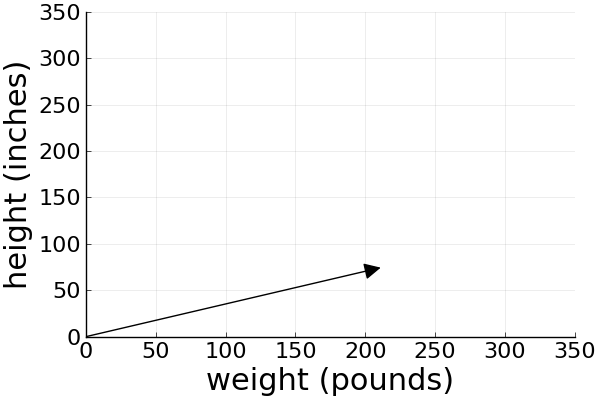
\includegraphics[width=0.4\textwidth]{vector.png}
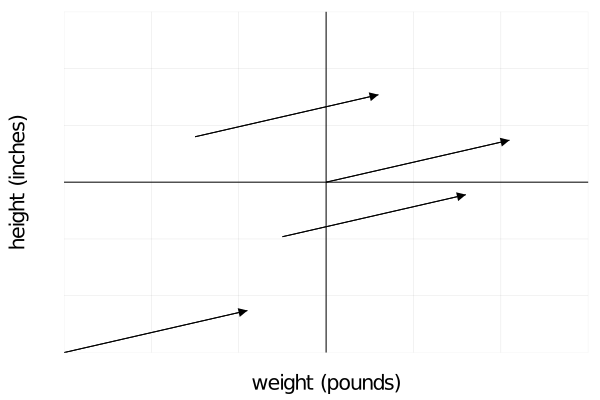
\includegraphics[width=0.58\textwidth]{vectors.png}
\caption{Left: a two-dimensional vector, depicted in a Cartesian plane. Right:
several copies of \textit{the same vector}, shown originating at various
points. They're considered ``the same'' vector because they all go in the same
direction and have the same length; the point they start at is irrelevant.}
\label{fig:vector}
\end{figure}

\index{magnitude (of a vector)}
\index{length (of a vector)}
\index{point of origin}
\index{direction (of a vector)}
\index{tail (of a vector)}
\index{tip (of a vector)}
\index{Stark, Arya}

You can see this illustrated on the right-hand side figure, where I've drawn
several copies of \textit{the same vector}. This may seem weird, but in terms
of pictures, here's how you want to think of it: \textbf{a vector has a
direction and a magnitude, but not a starting point}. The direction is the
specific angle in which it points, and (for now) we use the word
``\textbf{magnitude}'' to mean how long the vector is from its \textbf{tail} to
its \textbf{tip}. (As Arya Stark would say, the tip is the ``pointy end'' with
the arrowhead.) Curiously, there are alternative ways of judging the length, or
magnitude, of a vector, which we'll revisit in section~\ref{sec:norms}.

\index{counter-clockwise}

In the case of Stephen's biometric vector, its direction is
east-by-northeast-ish (about 19.4\textdegree\ counter-clockwise from the
$x$-axis) and its magnitude is 222.6. But it doesn't have any intrinsic ``point
of origin''; it's just an arrow pointing this-a-way and yea-far, no matter
where it might be anchored.

\index{mosquito}

Interestingly, the word \textit{vector} comes from a root meaning ``to carry.''
You may have heard people describe mosquitoes as being ``vectors'' for a
particular disease -- this means that they carry that disease. By thinking of a
vector as an arrow like in Figure~\ref{fig:vector}, the ``carry''
interpretation might start to make sense. A vector can represent a
transposition from one point to another. If I grew 74 inches taller and gained
210 more pounds, my point on the Cartesian plane would move in the direction
and the distance of that arrow.

\subsection{Don't visualize this}

Now that was all for \textit{two} dimensions. What about vectors with three, or
five, or even twenty dimensions? Well, for the three-dimensional case you can
indeed draw a 3-d figure with three axes, and plot three-dimensional points on
it. It turns out that most humans, though, are positively horrible at
interpreting such plots. And when you move beyond three dimensions, it's
utterly hopeless. (A friend of mine in fourth grade claimed he could visualize
four dimensions in his head, but I didn't believe him and still don't.)

But importantly, that doesn't mean we won't ever deal with higher-dimensional
vectors. In fact, vectors with lots and lots of dimensions will come up
constantly for us in this book -- believe it or not, we'll do an example where
the vectors have 50,000 dimensions! :-O

Don't worry; this won't make your head explode. In fact, it's a lot easier than
you might think to work with very high-dimensional vectors. Consider the
example I gave above about tracking a company's stock price every day for a
year. That's just a list of 365 numbers, all in a row. How hard is that to
imagine?

To work with vectors of more than three dimensions, you only have to do one
thing: give up trying to visualize them in a geometric space. As I'll describe
in the next section, it only occasionally makes sense to think about vectors
geometrically anyway; much of the time, we'll simply think of them as
quantities that have more than one component, unlike their simple brethren the
scalars.

\smallskip

Finally, the notation we'll use for vector variables. Instead of putting the
variable name in italics, we'll put it in bold-face with an arrow on the top of
it, like this: $\overrightarrow{\textbf{x}}$. The individual components of the
vector will be listed in boxies (square-brackets) like this: $[\ -2\ \ 5.9\ \
17\ \ -3\ ]$. So, if we define $\overrightarrow{\textbf{stephen}}$ as the
vector with my height and weight in it, we would write:

\vspace{-.15in}

\begin{align*}
\overrightarrow{\textbf{stephen}} = [\ 210\ \ 74 \ ].
\end{align*}

\medskip

\section{Five ways to think about vectors}

\begin{figure}[ht]
\centering
\includegraphics[width=1\textwidth]{fiveWays.pdf}
\caption{Five ways to think about a vector.}
\label{fig:fiveWays}
\end{figure}


In the mathematical writings you'll encounter, computer scientists use the word
``vector'' in a variety of ways. They're all ultimately compatible with each
other, but they can seem disorientingly different at first. Really, it's a
tribute to how powerful the vector concept is that people use them in so many
ways for so many different things.

I'm going to suggest that there are \textit{five} different ways to think about
a vector, and I'm going to arrange these ways on a continuum from ``concrete''
to ``abstract.'' This spectrum is depicted in Figure~\ref{fig:fiveWays}.

Let's take it from the bottom.

\subsection{1. A sequence of two coordinates}

\index{coordinate}
\index{element}
This is the height-weight example, in which something like
$\overrightarrow{\textbf{stephen}}$ is an ordered pair that can easily be
visualized on a two-dimensional Cartesian plane. Because of this plotting
aspect, I'll often call the two parts of the vector \textbf{coordinates}, but
as we create vectors with more pieces I'll more often call them
\textbf{elements}. These terms mean the same thing -- they both refer to the
individual components of the vector.

\index{index number}

We will need a way to select one of the coordinates individually, and for that
we use an \textbf{index number} (sometimes abbreviated to simply
``\textbf{index},'' the plural of which is ``indices.'') As you can see in
Figure~\ref{fig:fiveWays}, I've put two smaller numbers directly below the two
coordinates of the bottom vector, to indicate that we call them ``coordinate
\#0'' and ``coordinate \#1.'' We'll also use the phrase ``\textbf{index into
the vector},'' where ``index'' is a verb. If we take that bottom-most vector,
and index into it at coordinate 1, we get the (scalar) value 93.

Notation-wise, if we have a two-dimensional vector called
$\overrightarrow{\textbf{bob}}$, we'll often write $bob_0$ for the value of the
first coordinate and $bob_1$ for the second.

As an aside, you might wonder why the coordinates are numbered 0 and 1 instead
of 1 and 2. The answer has to do with the fact that we'll be using Python in
this book. Every programming language has a way of indexing into its
vector-like objects, and Python, Java, and C++ all begin indexing with the
number 0. There are actually some good reasons for this, which I won't get
into. It's not universally embraced, however; languages like R and Julia start
their indexing at 1. Go figure.

\index{tail (of a vector)}
\index{tip (of a vector)}

Geometrically, we can compute a vector's direction and magnitude using
trigonometry. Figure~\ref{fig:directionMag} shows a vector
$\overrightarrow{\textbf{v}} = [\ 9 \ \ 21\ ]$ pictorially. Its $0^\text{th}$
coordinate (a.k.a. $v_0$) is 9, measured on the $x$-axis, and $v_1$ is 21.
Traditionally, a two-dimensional vector's magnitude is called $r$ (for
``radius,'' I think, although don't think about that too hard) and its
direction is called $\theta$ (``theta''). The magnitude is just the crow-flies
distance from the vector's \textbf{tail} to its \textbf{tip} (computed using
the Pythagorean Theorem) and the direction is the arctangent of the
rise-over-run. In equations:

\vspace{-.25in}
\begin{align*}
r &= \sqrt{v_0^2 + v_1^2} \\
\theta &= \tan^{-1} \frac{v_1}{v_0} \\
\end{align*}
\vspace{-.55in}

\begin{figure}[ht]
\centering
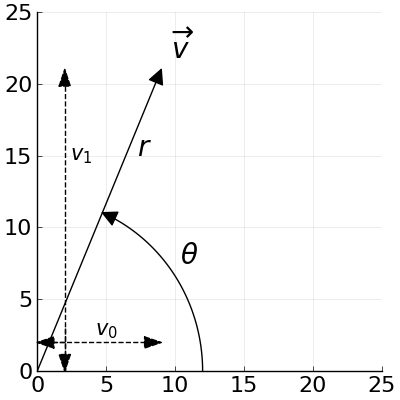
\includegraphics[width=.7\textwidth]{directionMag.png}
\caption[.]{The direction ($\theta$) and magnitude ($r$) of the vector
$\overrightarrow{\textbf{v}} = [\ 9 \ \ 21\ ]$. The direction $\theta$ is the
angle that $\overrightarrow{\textbf{v}}$ makes counter-clockwise with the
$x$-axis, and the magnitude is the length of the line.}
\label{fig:directionMag}
\end{figure}
\smallskip

\index{polar coordinates}
\index{Cartesian coordinates}

In this case, $r$ works out to 22.8 and $\theta$ is 66.8\textdegree. Think
about this, too: if, instead of giving you the values of $v_0$ and $v_1$, I
instead gave you the values of $r$ and $\theta$, you'd still have \textit{all
the information about the vector}, just in a different form. These are
sometimes called the \textbf{polar coordinates} of a vector, instead of the
\textbf{Cartesian coordinates}. The polar coordinates are usually written as
``$22.8 \measuredangle 66.8$\textdegree,'' which is the same vector as $[\ 9 \
\ 21 \ ]$, just written in a different way.

Anyway, I put this way of thinking about vectors at the extreme ``concrete''
end of the spectrum, because it's so nuts-and-bolts and easy to visualize. As
we ascend up the hierarchy, things will get less and less visualizable.


\subsection{2. A sequence of more than two coordinates}

As I mentioned earlier in this chapter, having more than two coordinates in a
vector isn't really all that weird...you simply have to give up any hope of
visualizing it geometrically. But it's easy enough to do: a list of four
numbers -- 89, 93, 70, and 133 -- is the most natural thing in the world. One
could imagine finding the sum of the elements, the maximum element, the number
of negative elements, or other more exotic things.

Again, our indexing starts at 0, and this time goes up to 3. Note what this
implies: if we have a vector with four elements, there is no element \#4! This
is a common pitfall for newcomers to the subject and to languages like Python.
If I have a vector with $n$ coordinates, those coordinates are numbered 0 up to 
$n-1$, but \textit{not} up to $n$.

\index{dimension}
Also note that the number of elements/coordinates is also the
\textbf{dimensionality} (number of dimensions) of the vector. Simply put, a
vector that has nine elements in it is called ``a 9-dimensional vector.''

\subsection{3. A collection with non-numeric indices}

At this point of the hierarchy, I change my nomenclature from ``sequence'' to
``collection.'' That's because here, we don't \textit{number} the elements of
our vector anymore but instead \textit{name} them. Thus there isn't any
meaningful order to the elements anymore -- instead of ``IQ \#0,'' ``IQ \#1,''
and so forth, we have ``Jezebel's IQ,'' ``Filbert's IQ,'' and the like. Nothing
super weird here, but things may be starting to look less and less math-y to
you.

\index{label}

I'll sometimes call the names of the elements \textbf{label}s.

% TODO: talk about how diff languages represent this in diff ways; with R, you
% can name the elements of a vector, whereas in Python, you'll need a dict.

\subsection{4. A collection with non-numeric elements}

And heck, if the indices don't have to be numbers, why would the elements need
to be? And indeed we will often have cause to work with vectors like the one in
step 4 of the hierarchy (Figure~\ref{fig:fiveWays}, p.~\pageref{fig:fiveWays}),
in which there's not a number in sight. This example holds the favorite colors
for each of our four friends, which are of course non-numeric.

\subsection{5. Just a ``thing''}

Finally, you won't see this usage of vectors until you get to some more
advanced math, but I'd be doing you a disservice if I didn't point it out here.
I remember the first time I read some research in which the author was going on
and on about ``vectors,'' and I was dreadfully confused because none of his
``vectors'' seemed to have any elements in them! I was like, ``what do you mean
\textit{vectors}, dude? Did your word processor auto-correct a different
word?''

\index{vector space}
\index{algebra@``an algebra''}

This computer scientist was treating ``vectors'' as whole objects, not even
considering what their elements were (or whether they even \textit{had} any
elements). He was working with an abstract notion called a \textbf{vector
space} which we'll touch on much later; for now I'll just tell you that it's
closely related to the notion of an algebra that we discussed in
Chapter~\ref{ch:intro}. He was taking advantage of some of the elegant results
presented later in this book, which are guaranteed to hold for whatever
mathematical objects you care to define, as long as you obey certain ground
rules -- whether those objects have any ``elements'' to them or not. I mention
this mostly to anchor your future self in solid ground the first time you
inevitably come across the use of ``vector'' as a very un-list-like thing.
You'll remember reading this, say to yourself ``ah yes -- Stephen warned me
once that the extreme abstract end of the continuum works like this,'' and
proceed with confidence. I won't say anything more about it in this book.

\section{And a vector is also a function}

\index{function}

Oh, and yet another way to think of vectors: as \textbf{function}s. We'll talk
about vectors as inputs to functions later in this book. But it's worth
recognizing at this point that a vector itself essentially \textit{is} a
function.

\index{domain}
\index{codomain}

You'll remember from Chapter 3 of \textit{Cool, Brisk Walk} that a function is
a mapping from a set of inputs to a set of outputs. Each member of the input
set (a.k.a. the ``domain'') is assigned a member of the output set
(``codomain'') as its value. (No member of the domain can be assigned to more
than one member of the codomain, but the reverse is not a constraint: multiple
members of the domain \textit{can} be assigned to the same member of the
codomain.)

Now consider this vector:

\begin{center}
\begin{tabular}{ccccccc}
$\overrightarrow{\textbf{x}} = [$ & 45 & -12 & 9 & 45 & 0 & $]$ \\
& \scriptsize{0} & \scriptsize{1} & \scriptsize{2} & \scriptsize{3} & \scriptsize{4}& \\
\normalsize
\end{tabular}
\end{center}
\vspace{-.15in}

It's a sequence of numbered elements, sure. But couldn't it just as easily be
interpreted as a function from index numbers to values? (See
Figure~\ref{vectorFunction1}.)

\begin{figure}[ht]
\centering
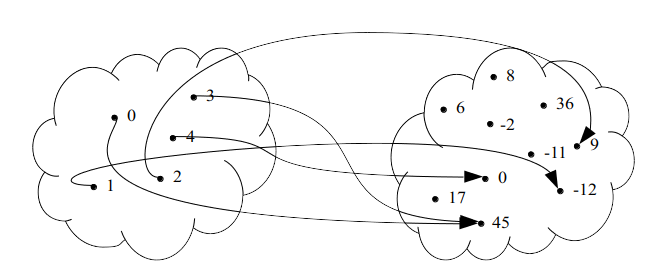
\includegraphics[width=1\textwidth]{vectorFunction1.png}
\caption[.]{The vector $\overrightarrow{\textbf{x}}$, interpreted as a function.}
\label{vectorFunction1}
\end{figure}

In function syntax, $\overrightarrow{\textbf{x}}(0) = 45$,
$\overrightarrow{\textbf{x}}(1) = -12$, $\overrightarrow{\textbf{x}}(3) = 45$,
and so on. It makes even more sense with a non-numeric vector like the
``favorite color'' example (Fig.~\ref{fig:fiveWays}), where
$\overrightarrow{\textbf{faveColor}}(\textrm{Biff}) = \textrm{blue}$ and
$\overrightarrow{\textbf{faveColor}}(\textrm{Betty Lou}) = \textrm{purple}$.
Instead of index numbers, the function's domain is comprised of the vector's
labels.

\index{ah-ha@``ah-ha"!''~moment}
\index{dictionary}
\index{hash table}
\index{array}
\index{associative array}
\index{list}
\index{vector}
\index{function}

I remember having a real ``ah-ha!''~moment the day I first realized that
vectors (called ``arrays'' or ``lists'' in some programming languages) were
really the same as key/value-pair-based associative arrays (also called
``dictionaries'' or ``hash tables'') with \textit{an index number as the key}.
Later, I had another ``ah-ha!''~and realized that both were equivalent to
functions as well, if you viewed the keys/indices as the function's domain and
the elements as the codomain. Wow. Sometimes it seems like the universe is
really all just one thing.

%Vectors in the wild
%
%
%time series
%
%temperatures over time
%
%
%
%items with attributes
%
%loan attributes: age, credit score, loan amount, salary
%
%
%
%MP3 file
%
%everything has to be in binary to be in a computer
%
%air displacement vs. time
%
%sampling
%
%
%
%image files
%
%BW vs color
%
%can do finding faces, brighten the image, whatever
%
%
%
%binary string of text
%
%plain-text, encrypt with key, to get cipher text
%
%
%
%
%Google, vector representation of web pages
%
%bag of words
%
%
%
%Emails, spam detectors
%
%
%
%matchmaker.com 
%
%
%
%Facebook:
%represent each vertex as a vector of people-he's-friends-with 
%
%
%Purchasing patterns, 
%recommender systems (collaborative filbert)
%
%
%
%system state, population growth


\section{Vector operations}

We're going to be combining scalars/vectors to yield other scalars/vectors like
literally all the time. The following three operations must be mastered until
you can do them in your sleep.

\subsection{Operation \#1: Scalar-vector multiplication}

What do you think you'd get if you multiplied a scalar like 2 by a vector like
$[\ 3\ \ 0\ \ 4\ ]$? As with all mathematics, we can define this operation to
be anything we want. A reasonable guess would be to take the scalar number of
copies of the vector, like so:

\vspace{-.15in}
\begin{align*}
2 \cdot [\ 3\ \ 0\ \ 4\ ] = [\ 3\ \ 0\ \ 4\ \ 3\ \ 0\ \ 4\ ] ? \quad  \quad
\textrm{NOPE}
\end{align*}
\vspace{-.15in}

But we're not doing to define it that way. Instead, we'll multiply the scalar
by each of the vector's elements individually, to get another vector with the
same number of elements:

\vspace{-.15in}
\begin{align*}
2 \cdot [\ 3\ \ 0\ \ 4\ ] = [\ 6\ \ 0\ \ 8\ ]
\end{align*}
\vspace{-.15in}

\index{scalar-vector multiplication}

This turns out to be more useful. So in general, a scalar $a$ times a vector
$\overrightarrow{\textbf{v}}$ will be:

\vspace{-.15in}
\begin{center}
\begin{framed}
\textbf{Scalar-vector multiplication:}
\begin{align*}
a \overrightarrow{\textbf{v}} = a [\ v_0\ \ v_1\ \ \dots \ \ v_{n-1}\ ] =
[\ a \cdot v_0\ \ a \cdot v_1\ \ \dots \ \ a \cdot v_{n-1}\ ],
\end{align*}
where $n$ is the number of elements in the vector.
\end{framed}
\end{center}
\vspace{-.15in}

Interestingly, there's no such thing (in common use) as ``scalar-vector
\textit{addition}.'' In other words, if someone tried to do this:

\vspace{-.15in}
\begin{align*}
2 + [\ 3\ \ 0\ \ 4\ ] = \ ??
\end{align*}
\vspace{-.15in}

\index{no can do@``no can do''}
we're simply going to say ``no can do.''

By the way, some programming languages (including Python) do give the
programmer a convenient shorthand by allowing them to type
$2 + [\ 3\ \ 0\ \ 4\ ]$ and get the value $[\ 5\ \ 2\ \ 6\ ]$. This isn't
considered a bona fide mathematical operation, though; just a notational
convenience.

\subsection{Operation \#2: Vector addition}

Adding two vectors together, though, is a perfectly acceptable enterprise,
provided that the vectors have the same number of elements. The way we do it is
to add each pair of elements together and produce another vector of the same
number of dimensions. In other words, adding $[\ 2\ \ 9\ ]$ to $[\ 4\ \ -2\ ]$
gives us:

\vspace{-.15in}
\begin{align*}
[\ 2\ \ 9\ ] + [\ 4\ \ -2\ ] = [\ 6\ \ 7\ ],
\end{align*}
\vspace{-.15in}

and in general:

\vspace{-.15in}
\begin{center}
\begin{framed}
\textbf{Vector addition:}
\begin{align*}
\overrightarrow{\textbf{x}} + \overrightarrow{\textbf{y}} &=
[\ x_0\ \ x_1\ \ \dots \ \ x_{n-1}\ ] +
[\ y_0\ \ y_1\ \ \dots \ \ y_{n-1}\ ] \\
&= [\ x_0 + y_0\ \ x_1 + y_1\ \ \dots \ \ x_{n-1} + y_{n-1}\ ],
\end{align*}
where $n$ is the number of elements in each vector.
\end{framed}
\end{center}
\vspace{-.15in}

An important issue arises in level 3 of our Figure~\ref{fig:fiveWays} hierarchy
(p.~\pageref{fig:fiveWays}). How do we add two vectors that aren't indexed by
number? Answer: we add the elements from each vector that correspond to the
same \textit{label}. And yes, the vectors must \textit{have} exactly the same
labels in order to be legitimately added in this way; otherwise, we call the
whole thing off. So:

\index{Mrs.~Peacock}
\index{Mr.~Green}
\index{Prof.~Plum}

\begin{center}
\begin{tabular}{ccccccccc}
[ & 3 & 5 & 8 & ] \ + \ [ & 1 & -6 & 4 & ] \ = \\
& \scriptsize{peacock} & \scriptsize{green} & \scriptsize{plum} & &
\scriptsize{peacock} & \scriptsize{green} & \scriptsize{plum} & \\
\normalsize
\end{tabular}
\vspace{-.15in}
\begin{tabular}{ccccc}
[ & 4 & -1 & 12 & ], \\
& \scriptsize{peacock} & \scriptsize{green} & \scriptsize{plum} & \\
\normalsize
\end{tabular}
\end{center}
\vspace{-.15in}

and

\index{Miss Scarlet}
\index{Mrs.~White}
\index{Col.~Mustard}

\begin{center}
\begin{tabular}{ccccccccc}
[ & 2 & 1 & 4 & ] \ + \ [ & 3 & 3 & 0 & ] \ = \\
& \scriptsize{scarlet} & \scriptsize{mustard} & \scriptsize{green} & &
\scriptsize{scarlet} & \scriptsize{white} & \scriptsize{plum} & \\
\normalsize
\end{tabular}

\index{no can do@``no can do''}
\vspace{-.15in}
``no can do.''
\end{center}
\vspace{-.15in}

\index{commutative}
\index{distributive}

\medskip
You can probably tell that vector addition is \textbf{commutative}, meaning
that whether we add $\overrightarrow{\textbf{x}}$ +
$\overrightarrow{\textbf{y}}$ or $\overrightarrow{\textbf{y}}$ +
$\overrightarrow{\textbf{x}}$, we get the same answer. It's also true that
vector addition, combined with scalar-vector multiplication, is
\textbf{distributive}. This means:

\vspace{-.15in}
\begin{align*}
a (\overrightarrow{\textbf{x}} + \overrightarrow{\textbf{y}}) &=
a \overrightarrow{\textbf{x}} + a \overrightarrow{\textbf{y}}
\end{align*}
\vspace{-.15in}
and

\vspace{-.15in}
\begin{align*}
(a + b) \overrightarrow{\textbf{x}} &=
a \overrightarrow{\textbf{x}} + b \overrightarrow{\textbf{x}}
\end{align*}
\vspace{-.15in}

for any scalars $a$ and $b$ and vectors $\overrightarrow{\textbf{x}}$ and
$\overrightarrow{\textbf{y}}$. This is a useful fact to know, which we'll
sometimes rely on.

\medskip

By the way, you might wonder whether vector subtraction is a thing, and it is:
in fact it turns out to just use scalar multiplication by $-1$. So:

\vspace{-.15in}
\begin{center}
$\overrightarrow{\textbf{x}} - \overrightarrow{\textbf{y}} =
\overrightarrow{\textbf{x}} + (-1 \overrightarrow{\textbf{y}}) =$ \\
$ [\ x_0 - y_0\ \ x_1 - y_1\ \ \dots \ \ x_{n-1} - y_{n-1}\ ]$.
\end{center}

For example, $[\ 5\ \ 2\ \ 7\ ] - [\ 1\ \ 4\ \ 7\ ]$ is just $[\ 4\ \ -2\ \ 0\ ]$.

\subsection{Operation \#3: Vector multiplication (dot product)}

\index{dot product}
\index{cross product}

Our third and final vector operation is the least intuitive of the three; at
least, it doesn't work the way I expected it to when I first learned it. It's
most commonly called the \textbf{dot product}.\footnote{There is at least one
other type of vector multiplication in common use, which we won't need in this
book. It's called the \textbf{cross product}, and is designated by a $\times$
instead of a $\cdot$. Interestingly, although the dot product is defined for
vectors of any number of dimensions, the cross product is only defined for
vectors of exactly three dimensions. (Not 2. Not 4. Only exactly 3.) Another
curious fact is that the cross product between two vectors gives you a vector
back, not a scalar like the dot product does.}

The first thing you have to wrap your head around is the fact that \textit{two
vectors multiplied together give you a scalar.} Yeah, no cap: if you multiply
an 18-dimensional vector by another 18-dimensional vector, you get back a
single lonely number.

Operationally, what happens is that you \textit{multiply} the corresponding
elements of the two vectors together, and then \textit{add} the result. So:

\vspace{-.15in}
\begin{align*}
[\ 7\ \ 8\ ] \cdot [\ 5\ \ 1\ ] = 7\cdot 5 + 8\cdot1 = 43
\end{align*}
\vspace{-.15in}

As with vector addition, we disallow taking the dot product of two vectors with
differing numbers of elements. Also, in the case of vectors with labels instead
of index numbers, we insist that the vectors have identical labels in order to
meaningfully dot-product them.

\index{dot product}
\begin{center}
\begin{framed}
\textbf{Vector multiplication (dot product):}
\begin{align*}
\overrightarrow{\textbf{x}} \cdot \overrightarrow{\textbf{y}} &=
[\ x_0\ \ x_1\ \ \dots \ \ x_{n-1}\ ] \cdot
[\ y_0\ \ y_1\ \ \dots \ \ y_{n-1}\ ] \\
&= x_0 \cdot y_0\ + x_1 \cdot y_1\ + \dots + x_{n-1} \cdot y_{n-1},
\end{align*}
where $n$ is the number of elements in each vector.
\end{framed}
\end{center}
\vspace{-.15in}

\index{commutative}

It should be obvious to you that the dot product operation is commutative:
$\overrightarrow{\textbf{x}} \cdot \overrightarrow{\textbf{y}}$ always gives
the same result as $\overrightarrow{\textbf{y}} \cdot
\overrightarrow{\textbf{x}}$.

\subsubsection{Why?}

Okay, now to address the elephant in the living room: \textit{why} would
mathematicians define vector multiplication in this way? What's the matter with
just multiplying corresponding elements and yielding a vector answer, like we
did with vector addition?

The answer is that the dot product as defined above is incredibly useful, much
more so than pairwise-multiplication will turn out to be. In fact, it's
possibly the single most important calculation in linear algebra: all kinds of
applications and more advanced computations use it as a building block.

To see this, consider the following question. What needs to be true about two
vectors in order for them to have a large dot product?

Your first inclination might be to answer ``the individual vector entries need
to be large.'' This is sort of true...but only sort of. Consider the following
two vectors:

\vspace{-.15in}
\begin{align*}
\overrightarrow{\textbf{a}} &= [\ 95\ \ 0\ 381\  ] \\
\overrightarrow{\textbf{b}} &= [\ 0\ \ 1056\ 0\  ] \\
\end{align*}
\vspace{-.15in}

Thar's som' mighty big entries in them vectors. Surely multiplying them
together would give a large result, right? No:

\vspace{-.15in}
\begin{align*}
[\ 95\ \ 0\ 381\ ] \cdot [\ 0\ \ 1056\ 0\ ] &= \\
95 \cdot 0 + 0 \cdot 1056 + 381 \cdot 0 &= 0.
\end{align*}
\vspace{-.15in}

We get zilch. By contrast, these two wimpy-looking vectors:

\vspace{-.15in}
\begin{align*}
\overrightarrow{\textbf{c}} &= [\ 1\ \ 2\ \ 5\ ] \\
\overrightarrow{\textbf{d}} &= [\ 0\ \ 2\ \ 7\ ] \\
\end{align*}
\vspace{-.15in}

do give a fairly hefty result:

\vspace{-.15in}
\begin{align*}
[\ 1\ \ 2\ \ 5\ ] \cdot [\ 0\ \ 2\ \ 7\ ] &= \\
1 \cdot 0 + 2 \cdot 2 + 5 \cdot 7 &= 39.
\end{align*}
\vspace{-.15in}

What's going on here?

\medskip

If you stare at the above calculations, you'll hit on a deep truth which is
worth pondering at length. And that is that in order for the dot product to be
large, the vectors must not only have large entries, but be large \textit{in
the same places.}

The reason that $\overrightarrow{\textbf{a}}$ and $\overrightarrow{\textbf{b}}$
had such a stunningly low dot product is that although they had large entries,
they were completely out of sync with each other. $\overrightarrow{\textbf{a}}$
had high values precisely where $\overrightarrow{\textbf{b}}$ had low ones, and
vice versa. On the other hand, even though the individual elements of
$\overrightarrow{\textbf{c}}$ and  $\overrightarrow{\textbf{d}}$ were pretty
small, they fit together nicely: for example, $\overrightarrow{\textbf{c}}$'s
largest entry and $\overrightarrow{\textbf{d}}$'s largest entry were in the
same place (element \#2), which led to a kind of synergy.

Consider how the dot product would change if we altered
$\overrightarrow{\textbf{d}}$ to be $[\ 7\ \ 2\ \ 0\ ]$ instead of $[\ 0\ \ 2\
\ 7\ ]$:

\vspace{-.15in}
\begin{align*}
[\ 1\ \ 2\ \ 5\ ] \cdot [\ 7\ \ 2\ \ 0\ ] &= \\
1 \cdot 7 + 2 \cdot 2 + 5 \cdot 0 &= 11.
\end{align*}
\vspace{-.15in}

Dang, we dropped from 39 all the way to 11 just by reordering the entries. 

\index{Jezebel}

This ability to judge roughly ``how aligned'' two vectors are comes up all the
time. Consider a dating website. Let's say that Jezebel, a heterosexual female,
signs up for a dating service and answers the questions on a compatibility
survey. She's asked, ``on a scale of 1 to 10, how much do you like action
movies? Outdoor hikes? Candlelight dinners? Reading mystery novels?'' Suppose
her answers are the following:

\begin{center}
\begin{tabular}{cccccc}
$\overrightarrow{\textbf{jezebel}}$ = [ & 5 & 2 & 10 & 2 & ] \\
& \scriptsize{action} & \scriptsize{hiking} & \scriptsize{candlelight} &
\scriptsize{mystery} & \\
\normalsize
\end{tabular}
\end{center}
\vspace{-.15in}

\index{Filbert}
\index{Wendell}
\index{Biff}

Now there are three eligible heterosexual bachelors on this site: Biff,
Filbert, and Wendell. They also took the survey, and came up with these
responses:

\begin{center}
\begin{tabular}{cccccc}
$\overrightarrow{\textbf{biff}}$ \quad \ = [ & 10 & 10 & 1 & 1 & ] \\
& \scriptsize{action} & \scriptsize{hiking} & \scriptsize{candlelight} &
\scriptsize{mystery} & \medskip \\

$\overrightarrow{\textbf{filbert}}$ \ = [ & 6 & 2 & 8 & 4 & ] \\
& \scriptsize{action} & \scriptsize{hiking} & \scriptsize{candlelight} &
\scriptsize{mystery} & \medskip \\

$\overrightarrow{\textbf{wendell}}$ = [ & 1 & 3 & 3 & 10 & ] \\
& \scriptsize{action} & \scriptsize{hiking} & \scriptsize{candlelight} &
\scriptsize{mystery} & \\
\normalsize
\end{tabular}
\end{center}
\vspace{-.15in}

The central question that \texttt{matchmaker.com} must ask is: which of these
three young gentlemen should be recommended to Jezebel?

\smallskip

The answer lies in the dot product. Just by eyeballing the survey results, you
can probably tell that Filbert is Jezebel's best match: he has high values in
roughly the same place that she does. If we compute the dot product of Jezebel
with each of the three guys, we see that the math bears that out:

\begin{align*}
\overrightarrow{\textbf{jezebel}} \cdot \overrightarrow{\textbf{biff}} &=
5 \cdot 10 + 2 \cdot 10 + 10 \cdot 1 + 2 \cdot 1 = 82 \\
\overrightarrow{\textbf{jezebel}} \cdot \overrightarrow{\textbf{filbert}} &=
5 \cdot 6 + 2 \cdot 2 + 10 \cdot 8 + 2 \cdot 4 = 122 \\
\overrightarrow{\textbf{jezebel}} \cdot \overrightarrow{\textbf{wendell}} &=
5 \cdot 1 + 2 \cdot 3 + 10 \cdot 3 + 2 \cdot 10 = 61 \\
\end{align*}

Since Filbert has the highest dot product with Jezebel, Filbert's vector is in
some sense ``more closely aligned'' with hers, reflecting their similar
interests. So our website will show Filbert's pic and profile to Jezebel.

\medskip

\index{Mr.~Right}

It might occur to you that someone could ``beat the system'' here by answering
10 on all their survey questions. After all, increasing the individual entries
in a vector can't \textit{hurt} its dot product with another vector; the worst
it could do is not help matters, if the second vector has a zero there. So
let's say the insidious Mr.~Right (?) creates an account on the system, and
answers:

\begin{center}
\begin{tabular}{cccccc}
$\overrightarrow{\textbf{mrright}}$ \quad \ = [ & 10 & 10 & 10 & 10 & ] \\
& \scriptsize{action} & \scriptsize{hiking} & \scriptsize{candlelight} &
\scriptsize{mystery} & \medskip \\
\normalsize
\end{tabular}
\end{center}
\vspace{-.15in}

Pairing him with Jezebel yields:

\begin{align*}
\overrightarrow{\textbf{jezebel}} \cdot \overrightarrow{\textbf{mrright}} &=
5 \cdot 10 + 2 \cdot 10 + 10 \cdot 10 + 2 \cdot 10 = 190 \\
\end{align*}

which blows away the competition. Mr.~Right can have any girl he wants, whether
or not they're truly compatible. There's a way to fix this, which we'll see
later in this chapter. For now, just grasp the main point that two vectors
having large entries in the same places tends to magnify their dot product.

%brownies / chippers / etc  example
%    first "how much of each ingredient would I need for these recipes"
%    then "how much would it cost at Wegmans to buy that list"
%
%
%dot product geometrically (three different orthogonal cases)
%    if they're orthogonal, their dot product is zero.
%    another way to compute dot product: magnitude of one vec * meg of other
%        * cos theta


\section{Norms and normalization}
\label{sec:norms}

    "size" "bigness" "magnitude" "length"
    magnitude / length

%    the l^n norm  (but don't use n if you also use n for # of vec elems)
%    l^2 norm -- Euclidean norm / Pythagorean Theorem / crow flies

%    more generally, n=3, n=4, n=193   (note: have to take abs value)
% manhattan / taxicab norm
% l^0 norm (number of non-zero entries in vector)
% l^inf norm, abs value of max element

%"Normalizing" -- dividing by the norm. (just want the magnitude)
%    [ 4 3 ] -> [ 4/5  3/5 ]
% only care about the direction
% now jezebel can't cheat with [ 10 10 10 10 10 ]. same as Chad, who answered
% [ 5 5 5 5 5 ].
